% !TeX root = ..

\section{
  Точное вычисление целевых функций
  в~задаче оптимизации маршрута резки
  на примере машины лазерной резки
  {\it ByStar~3015}
}
\label{sect:2.1}
\setcounter{equation}{0}

Как мы уже  отмечали в \ref{sect:1.2}
для задачи оптимизации маршрута резки (\ref{problem-statement})
проблема точного вычисления целевых функций времени резки и стоимости резки,
определяемых, в частности, формулами (\ref{cutting-time}) и (\ref{cutting-cost}):
$$
T_{cut} = \frac{L_{on}}{V_{on}} + \frac{L_{off}}{V_{off}} +N_{pt} \cdot t_{pt}
$$
$$
F_{cost}=
L_{on} \cdot C_{on} +
L_{off} \cdot C_{off} +
N_{pt} \cdot C_{pt}
$$
является малоисследованной.
Ниже будут приведены результаты исследований,
проведенных А. Ф. Таваевой на предприятии
АО <<Производственное объединение <<Уральский оптико-механический завод>>
имени Э. С. Яламова>>
(Екатеринбург)
на машине лазерной резки
{\it ByStar 3015}.
Более подробно результаты этих исследований изложены в
\cite{intro45,intro46,intro47}.

% !TeX root = ..

\subsection{
  Вычисление фактического времени лазерной резки
  машины с~ЧПУ
  в~зависимости от параметров управляющей программы
  и~технологических факторов процесса резки
}
\label{sect:2.1.1}

Неточность вычисления фактического времени резки
$T_{cut}$
связана с тем, что скорость рабочего хода машины с ЧПУ
$V_{on}$,
программируемая в управляющей программе как константа,
фактически таковой не является и может меняться
в зависимости от различных технологических факторов,
а также характеристик спроектированной управляющей программы.
В частности, было установлено,
что при увеличении числа кадров в управляющих программах
резки разных наборов заготовок,
имеющих один и тот же суммарный периметр контуров,
фактическая средняя скорость резки падает.
Причины, по которым УП могут содержать большое количество кадров,
в основном, связаны с тем, что контуры со сложной геометрией
(например, сплайны) при конвертации из
{\it CAD}-системы в
{\it CAM}-модуль из-за разницы в геометрических форматах файлов
разбиваются на большое число геометрических примитивов
(например, на отрезки прямых и дуги окружностей),
т. е. аппроксимируются более простыми геометрическими примитивами.
Разница в форматах, в свою очередь,
вызвана тем, что практически все системы ЧПУ
оснащаются только линейными и круговыми интерполяторами.
Как правило, аппроксимация сложной геометрии сводится
именно к линейной аппроксимации.
Иногда конвертеры
{\it CAD}-файлов аппроксимируют отрезками прямых
даже дуги окружностей, хотя в этом нет необходимости,
если система ЧПУ поддерживает круговую интерполяцию.

Ниже приведены некоторые практические результаты
по определению зависимости скорости рабочего хода
инструмента лазерного комплекса
{\it ByStar 3015}
от количества кадров управляющей программы.

Исследования были проведены для следующих материалов:
Ст10кп ($\Delta$~= 1--10 мм)
и АМг3М ($\Delta$ = 1--5 мм).
Для проведения вычислительных экспериментов были разработаны
150 тестовых УП для резки различных фигурных заготовок с числом кадров
$n \in \overline{10,5000}$
для материала Ст10кп
и 150 УП -- для материала
АМг3М с числом кадров
$n \in \overline{10,2000}$.

Статистический материал был обработан в программе
{\it Mathcad},
и с помощью метода наименьших квадратов были построены
аппроксимирующие функции для зависимости скорости
рабочего хода инструмента
$V_{on}$
от количества кадров в спроектированной УП.
По результатам эксперимента были сделаны следующие выводы.

\begin{enumerate}
\item
Фактическая средняя скорость рабочего хода режущего инструмента
$V_{on}$
является монотонно убывающей функцией от числа кадров УП
(рис.~\ref{amg3m+10kp}).

\begin{figure}[p]
  \centering
  \subfigure[]{
    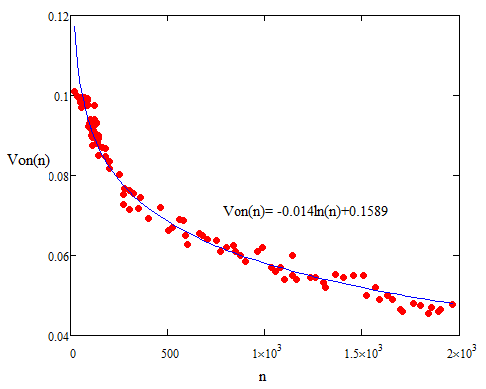
\includegraphics[width=0.77\textwidth]{amg3m.png}
    \label{amg3m}
  }
  \subfigure[]{
    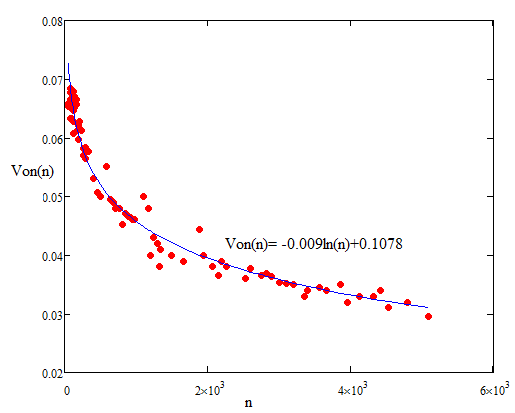
\includegraphics[width=0.77\textwidth]{10kp.png}
    \label{10kp}
  }
  \caption{
    Изменение скорости режущего инструмента
    на рабочем ходу: \\
    {\it а} -- АМг3М, $\Delta$ = 1 мм ($n \in \overline{10,2000}$); \\
    {\it б} -- Ст10кп, $\Delta$ = 3 мм ($n \in \overline{10,5000}$)
  }
  \label{amg3m+10kp}
\end{figure}

\item
Заданная в УП скорость
$V_{on}$
совпадает с фактической средней скоростью
при достижении числа кадров некоторого порогового значения $N$.
Когда количество кадров в УП меньше порогового значения $n<N$,
то фактическая скорость выше заданной,
а при увеличении числа кадров больше порогового $n>N$
-- может существенно снижаться
(в проведенных экспериментах снижение средней
фактической скорости режущего инструмента по сравнению
с заданным в УП значением доходило до 70 \%).

\item
Пороговое значение различно для разных марок материала и толщин.

\end{enumerate}

Для изложения результатов вычислительных экспериментов
введем следующие обозначения:
пусть
$n$ -- число кадров в УП,
$V_\text{факт}$ -- фактическая средняя скорость режущего инструмента при заданной скорости $V_{on}$,
$N$ -- число кадров (пороговое значение), для которого $V_\text{факт}=V_{on}$;
$\sum \varepsilon_n^2$ -- сумма квадратов отклонений исходных значений
скорости режущего инструмента и значений аппроксимирующей функции $V_{on}(n)$
в этих точках.

При аппроксимации точечных графиков
зависимости фактической скорости
$V_\text{факт}$
от числа кадров $n$
в УП аппроксимирующими кривыми в
{\it Mathcad}
для всех значений исследуемых марок материала и толщин материала было установлено,
что сходимость
$\sum \varepsilon_n^2 \to 0$
достигается при аппроксимации экспериментальных данных логарифмической функцией.

Аналогичные результаты были получены для материала
АМг3М $\Delta$~=~2--5 мм
и 10кп $\Delta$ = 1--10 мм.
Обобщенные результаты для всех исследованных марок материала и толщин
приведены в табл.~\ref{v-formulae}.

При использовании материала других марок
необходимо проведение дополнительных исследований
либо использование имеющихся данных по материалу
с близкими физическими свойствами.

Рассмотрим пример оптимизации времени резки
$T_{cut}$
(\ref{cutting-time})
при резке 15 фигурных заготовок
(материал АМг3М, $\Delta$ = 1 мм).
Раскройная карта
(рис.~\ref{amg-cutting})
содержит 15 заготовок двух типоразмеров,
при этом количество граничных контуров заготовок равно 19.
Каждый контур вырезается с помощью резки
<<по замкнутому контуру>>.
С целью сокращения множества допустимых решений
задачи множество возможных точек врезки было
ограничено конечным множеством
(задача $GTSP$),
состоящим из 55 точек
(обозначены маленькими квадратиками;
соответствующие точки выключения инструмента обозначены крестиками).
Для решения задачи использован точный алгоритм на основе ДП.
УП резки для данного примера содержат 120~команд или кадров
(т. е. $n=120$),
которые включают команды перемещения инструмента
для резки контуров
(с учетом разбиения каждого контура на несколько геометрических примитивов)
на рабочем ходу,
команды перемещения инструмента на холостом ходу
и ряд технологических команд.
Скорость рабочего хода инструмента, заданная в УП,
$V_{on}=0,1$ м/с.

\begin{table}[H]
  \caption{
    Обобщенная таблица формул
    для вычисления рабочей скорости инструмента
    на~лазерном комплексе
    {\it ByStar 3015}
    }
  \label{v-formulae}
  \centering
  \begin{tabular}{l|l|l}
    \hline
    Материал & Толщина, мм & Формула расчета $V_{on}$ \\
    \hline
    \multicolumn{3}{c}{$n\in\overline{10,5000}$} \\
    10кп & 1 & $V_{on} = -0,024 \ln n+0,245$ \\
    10кп & 2 & $V_{on} = -0,015 \ln n+0,1686$ \\
    10кп & 3 & $V_{on} = -0,009 \ln n+0,1078$ \\
    10кп & 3,5 & $V_{on} = -0,006 \ln n+0,0756$ \\
    10кп & 4 & $V_{on} = -0,006 \ln n+0,0709$ \\
    10кп & 8 & $V_{on} = -0,003 \ln n+0,0442$ \\
    10кп & 10 & $V_{on} = -0,002 \ln n+0,0365$ \\
    \multicolumn{3}{c}{$n\in\overline{10,2000}$} \\
    АМг3М & 1 & $V_{on} = -0,014 \ln n+0,1589$ \\
    АМг3М & 1,5 & $V_{on} = -0,001 \ln n+0,011$ \\
    АМг3М & 3 & $V_{on} = -0,004 \ln n+0,0672$ \\
    АМг3М & 4 & $V_{on} = -0,001 \ln n+0,0301$ \\
    АМг3М & 5 & $V_{on} = -6\cdot 10^{-4} \ln n+0,0177$ \\
    \hline
  \end{tabular}
\end{table}

На рис. \ref{amg-cutting+optimal}, {\it а}
показан маршрут резки
(перемещение инструмента на холостом ходу показано стрелками),
для которого значение целевой функции
$T_{cut}$ (\ref{cutting-time})
при
$V_{on}=0,1$ м/с
составляет
$T_{cut}=126,27$ с.
Однако фактическое время резки по управляющей программе,
составленной для этого маршрута,
оказалось (как и ожидалось)
значительно больше,
поскольку число кадров в программе ($n=120$)
значительно больше порогового значения $N=70$
для материала
АМг3М
$\Delta$ = 1 мм.

При использовании значения
$V_{on}=-0,014 \ln n + 0,1589$
(табл.~\ref{v-formulae})
в целевой функции (\ref{cutting-time})
оптимизационная процедура ДП
дает другое оптимальное решение задачи,
которое показано на рис.~\ref{amg-cutting+optimal}, {\it б}.
Тогда среднее фактическое значение
рабочей скорости инструмента при $n=120$
составило
$V_{on}=0,0919$ м/с.
В свою очередь,
для оптимального маршрута резки значение времени резки составило
$T_{cut}=141,38$ с.

\begin{figure}[H]
  \centering
  \subfigure[]{
    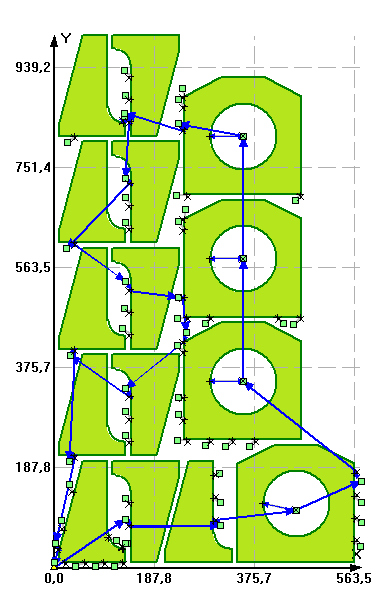
\includegraphics[width=0.45\textwidth]{amg-cutting.png}
    \label{amg-cutting}
  }
  \subfigure[]{
    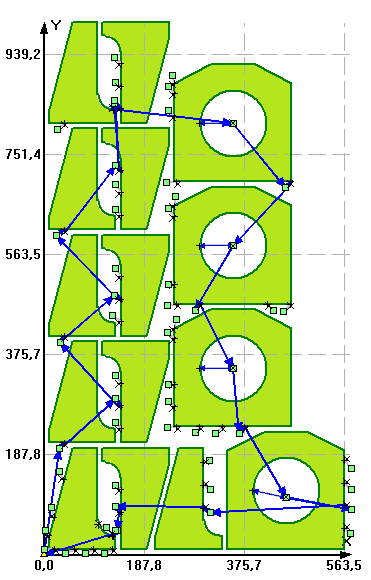
\includegraphics[width=0.45\textwidth]{amg-optimal.png}
    \label{amg-optimal}
  }
  \caption{
    Раскройная карта и оптимальный по времени маршрут
    перемещения режущего инструмента для 15 заготовок
    (материал АМг3М, $\Delta$ = 1 мм): \\
    {\it а} -- $V_{on}=const=0,1$ м/с; \\
    {\it б} -- $V_{on}=-0,014 \ln n + 0,1589$
  }
  \label{amg-cutting+optimal}
\end{figure}

Таким образом,
точное вычисление целевой функции для
данного примера обеспечило не только
точное вычисление значения экстремума
целевой функции, но и другой (правильный)
результат поиска оптимального маршрута резки,
полученный  с учетом числа кадров УП.

Этот пример иллюстрирует необходимость
получения таблиц типа табл.~\ref{v-formulae}
при решении конкретных оптимизационных задач
маршрутизации инструмента машин листовой резки с ЧПУ.

% !TeX root = ../mat_mod2.tex

\subsection{
  Вычисление стоимости резки заготовок
  на машине с~ЧПУ в режиме моделирования процесса резки
}
\label{sect:2.1.2}

Другая проблема точного вычисления целевой функции
при оптимизации маршрута резки связана
с поиском адекватных значений стоимости в формуле (\ref{cutting-cost}):
$$
F_{cost}=
L_{on} \cdot C_{on} +
L_{off} \cdot C_{off} +
N_{pt} \cdot C_{pt}
.
$$

Напомним:
$L_{on}$ – длина реза с включенным режущим инструментом;
$C_{on}$ – стоимость единицы пути с включенным режущим инструментом;
$L_{off}$ – длина переходов с выключенным режущим инструментом (холостой ход);
$C_{off}$ – стоимость единицы пути с выключенным режущим инструментом;
$N_{pt}$ – количество точек врезки,
$C_{pt}$ – стоимость одной точки врезки.

Рассмотрим вопрос точного вычисления
стоимости лазерной резки в задаче
оптимизации маршрута режущего инструмента
применительно к машине лазерной резки (тип лазера: СО$_2$)
с ЧПУ на примере машины
{\it ByStar3015}.

Проблема точного вычисления целевой функции
при оптимизации маршрута резки связана с
поиском адекватных значений стоимости
$F_{cost}$,
вычисление которой зависит от параметров
$C_{on}, C_{off}, C_{pt}$.

Для расчета
$C_{on}$
введем следующие обозначения для стоимостных параметров,
вычисляемых на 1 м рабочего хода инструмента:
$C_\text{расх}$ -- стоимость расходных материалов (например, сопло, защитное стекло, газовые трубки);
$C_\text{тех}$ -- стоимость технологического газа (азот или кислород в зависимости от типа обрабатываемого материала);
$C_\text{лаз}$ -- стоимость лазерного газа (при работе на машине с ЧПУ на проточном газовом лазере),
$C_\text{э/э}^{on}$ -- стоимость электроэнергии;
$C_\text{зп}^{on}$ -- затраты, связанные с заработной платой сопровождающего персонала;
$C_\text{А}^{on}$ -- амортизация оборудования.
Тогда в общем виде
$C_{on}$
будем вычислять по следующей формуле:
\begin{equation}
  C_{on} =
  C_\text{э/э}^{on} +
  C_\text{тех} +
  C_\text{лаз} +
  C_\text{расх} +
  C_\text{зп}^{on} +
  C_\text{А}^{on}
  .
  \label{c-on}
\end{equation}

Для вычисления значений
$C_{on}, C_\text{э/э}^{on}, C_\text{тех},
C_\text{лаз}, C_\text{расх}, C_\text{зп}^{on}, C_\text{А}^{on}$
введем дополнительные обозначения:
$t_{on}$ -- время, затрачиваемое на единицу длины рабочего хода инструмента, ч;
$P_{on}$ -- затраты электроэнергии за один час работы лазерного комплекса на рабочем ходу, кВт/ч;
$V_\text{тех}$ -- расход технологического газа, м$^3$/ч;
$V_\text{лаз}$ -- расход лазерного газа, м$^3$/ч;
$C_\text{э/э}$ -- стоимость электроэнергии за 1 кВт;
$C_{\text{лазМ}^3}$ -- стоимость 1м$^3$ лазерного газа;
$C_{\text{техМ}^3}$ -- стоимость 1м$^3$ технологического газа;
$C_\text{расхЕд}$ -- стоимость единицы расходных материалов;
$t_\text{расхСрок}$ -- срок службы расходных материалов;
$C_\text{зп}$ -- стоимость 1~ч работы обслуживающего персонала;
$A$ -- амортизация за 1~ч работы лазерного комплекса, руб;
$N$ -- срок полезного использования оборудования, год;
$C_\text{оборуд}$ -- первоначальная стоимость лазерного комплекса.
Тогда
$C_{on}, C_\text{э/э}^{on}, C_\text{тех},
C_\text{лаз}, C_\text{расх}, C_\text{зп}^{on}, C_\text{А}^{on}$
вычислим по следующим формулам:
\begin{equation}
  C_\text{э/э}^{on} =
  P_{on} t_{on}   C_\text{э/э}
  ,
  \label{c-on-ee}
\end{equation}

\begin{equation}
  C_\text{тех} =
  V_\text{тех} C_{\text{техМ}^3} t_{on}
  ,
  \label{c-on-teh}
\end{equation}

\begin{equation}
  C_\text{лаз} =
  V_\text{лаз} C_{\text{лазМ}^3} t_{on}
  ,
  \label{c-on-laz}
\end{equation}

\begin{equation}
  C_\text{расх} =
  \frac{C_\text{расхЕд}}{t_\text{расхСрок}}
  ,
  \label{c-on-rasx}
\end{equation}

\begin{equation}
  C_\text{зп}^{on} =
  C_\text{зп} t_{on}
  ,
  \label{c-on-zp}
\end{equation}

\begin{equation}
  C_\text{А}^{on} =
  \frac{1}N \frac{C_\text{оборуд}}{1920} t_{on}
  .
  \label{c-on-A}
\end{equation}

Параметр
$C_\text{тех}$
необходимо учитывать при расчете стоимости резки
только в тех случаях,
когда применяется вспомогательный рабочий газ
(кислород, азот в зависимости от типа обрабатываемого материала)
для увеличения скорости резки,
возможности обработки материалов более высоких толщин
и для сокращения затрат электроэнергии.
Расход газа зависит от диаметра используемого сопла и давления газа.

Для расчета
$C_{off}$
введем следующие обозначения параметров,
вычисляемых на 1~м холостого хода режущего инструмента:
$P_{off}$ -- затраты электроэнергии за 1~ч работы лазерного комплекса на холостом ходу, кВт/ч;
$t_{off}$ -- время, затрачиваемое на один метр холостого хода инструмента, ч.
Тогда
\begin{equation}
  C_{off} =
  P_{off} t_{off} C_\text{э/э}
  + C_\text{зп} t_{off}
  + \frac{1}N \frac{C_\text{оборуд}}{1920} t_{off}
  .
  \label{c-off}
\end{equation}

Аналогично для расчета
$C_{pt}$
введем следующие обозначения для стоимостных параметров,
вычисляемых на одну точку врезки:
$C_\text{э/э}^{pt}$ -- стоимость электроэнергии;
$C_\text{расх}^{pt}$ -- стоимость расходных материалов;
$C_\text{лаз}^{pt}$ -- стоимость лазерного газа;
$C_\text{тех}^{pt}$ -- стоимость технологического газа,
$C_\text{зп}^{pt}$ -- затраты, связанные с заработной платой сопровождающего персонала;
$C_\text{А}^{pt}$ -- амортизация оборудования.
Тогда
\begin{equation}
  C_{pt} =
  C_\text{э/э}^{pt} +
  C_\text{расх}^{pt} +
  C_\text{лаз}^{pt} +
  C_\text{тех}^{pt} +
  C_\text{зп}^{pt} +
  C_\text{А}^{pt}
  .
  \label{c-pt}
\end{equation}

Для вычисления значений
$C_\text{э/э}^{pt}, C_\text{расх}^{pt}, C_\text{лаз}^{pt}, C_\text{тех}^{pt}$
введем дополнительные параметры:
$P_{pt}$ -- затраты электроэнергии на одну точку врезки, кВт/ч;
$t_{pt}$ -- время, затрачиваемое на одну точку врезки, ч.
Тогда
\begin{equation}
  C_\text{э/э}^{pt} =
  P_{pt} t_{pt}   C_\text{э/э}
  ,
  \label{c-pt-ee}
\end{equation}

\begin{equation}
  C_\text{тех}^{pt} =
  V_\text{тех} C_{\text{техМ}^3} t_{pt}
  ,
  \label{c-pt-teh}
\end{equation}

\begin{equation}
  C_\text{лаз}^{pt} =
  V_\text{лаз} C_{\text{лазМ}^3} t_{pt}
  ,
  \label{c-pt-laz}
\end{equation}

\begin{equation}
  C_\text{расх}^{pt} =
  \frac{C_\text{расхЕд}}{t_\text{расхСрок}}
  ,
  \label{c-pt-rasx}
\end{equation}

\begin{equation}
  C_\text{зп}^{pt} =
  C_\text{зп} t_{pt}
  ,
  \label{c-pt-zp}
\end{equation}

\begin{equation}
  C_\text{А}^{pt} =
  \frac{1}N \frac{C_\text{оборуд}}{1920} t_{pt}
  .
  \label{c-pt-A}
\end{equation}

При расчете стоимости одной точки врезки параметр
$C_\text{лаз}^{pt}$
необходимо учитывать только при обработке материала
на проточном газовом лазере.
Параметр
$C_\text{тех}^{pt}$
необходимо учитывать при расчете себестоимости резки только в тех случаях,
когда применяется вспомогательный рабочий газ.

Тогда целевую функцию стоимости резки (\ref{cutting-cost})
можно записать в следующем виде:
\begin{multline}
  F_{cost} =
  L_{on} \left(
    C_\text{э/э}^{on} +
    C_\text{тех} +
    C_\text{лаз} +
    C_\text{расх} +
    C_\text{зп}^{on} +
    C_\text{А}^{on}
      \right) +
  \\
  L_{off} C_{off} +
  \\
  N_{pt} \left(
    C_\text{э/э}^{pt} +
    C_\text{расх}^{pt} +
    C_\text{лаз}^{pt} +
    C_\text{тех}^{pt} +
    C_\text{зп}^{pt} +
    C_\text{А}^{pt}
      \right)
  .
  \label{c-full}
\end{multline}

К основным расходным материалам и запчастям
для газового лазера можно отнести:
поворотные зеркала, фокусирующие линзы,
защитные стекла, сопла, юстировочные узлы,
газовые трубки.
К основным расходным материалам для
волоконного лазера можно отнести:
сопла, защитные стекла, фокусирующие линзы.
А для случая применения твердотельных лазеров
выделяют следующие основные расходные материалы и запчасти:
лампы оптической накачки, защитные стекла, зеркала,
квантрон, активный элемент.
Следует отметить, что стоимость расходных материалов
может изменяться в зависимости от фактических сроков
службы расходных материалов,
которые зависят от качества используемого газа,
опыта персонала, эксплуатирующего лазерный станок.
Следует отметить, что
$C_\text{расхЕд}$
зависит от ценообразования, курса доллара
({\it USD}) и евро
({\it EUR}),
а параметры
$C_\text{э/э}$,
$C_{\text{лазМ}^3}$ и
$C_{\text{техМ}^3}$
зависят от цен, которые устанавливает поставщик услуг,
поэтому при расчете
$F_{cost}$
для конкретных производственных задач,
изменения цен целесообразно учитывать,
используя изменяющиеся в зависимости от перечисленных
факторов таблицы стоимостных параметров в
{\it MS Excel}.
В частности, была создана сводная таблица в
{\it MS Excel}
для расчета себестоимости лазерной резки по разработанной
выше методике для газового СО$_2$
лазерного комплекса
{\it ByStar 3015}
для следующих материалов:

\begin{itemize}
\item
нержавеющая сталь (на примере 12Х18Н10Т) толщиной $\Delta$ = 1 -- 10 мм;
\item
углеродистая сталь (на примере 10кп) толщиной $\Delta$ = 1 -- 15 мм;
\item
алюминий и его сплавы (на примере {\it АМг3М}) толщиной $\Delta$ = 1 -- 5 мм.
\end{itemize}

Были определены значения основных стоимостных характеристик
$C_{on}$, $C_{off}$, $C_{pt}$
с учетом всех перечисленных параметров, приведенных в
(\ref{c-on}) -- (\ref{c-pt-A}).
В табл. \ref{c-table} приведены значения стоимости
одного погонного метра лазерного реза при максимальной
$C_{on}^{max}$
и минимальной
$C_{on}^{min}$
возможной рабочей скорости перемещения режущего инструмента
$V_{on}$
в зависимости от требуемого качества изготовления деталей.

\begin{table}
  \caption{
    Значения основных стоимостных параметров
    при вычислении целевой функции для
    CO$_2$ лазерного комплекса
    {\it ByStar3015}
  }
  \label{c-table}
  \centering
  \begin{tabular}{c*{5}{|r}}
    \hline
    Материал & Толщина, мм & $C_{on}^{max}$, руб & $C_{on}^{min}$, руб & $C_{off}$, руб & $C_{pt}$, руб \\
    \hline
    10кп	& 1	& 5.3	& 7.5	& 0.42	& 0.7 \\
    10кп	& 1.2	& 6.6	& 9.5	& 0.42	& 1.0 \\
    10кп	& 1.5	&  6.6	& 9.5	& 0.42	& 1.1 \\
    10кп	& 2	& 8.1	& 11.7	& 0.42	& 1.3 \\
    10кп	& 2.5	&	9.7	& 14.0	& 0.42	& 1.5 \\
    10кп	& 3	& 12.0	& 17.4	& 0.42	& 1.6 \\
    10кп	& 3.5	&	13.3	& 19.0	& 0.42	& 1.6 \\
    10кп	& 3.9	&	13.3	& 19.0	& 0.42	& 1.9 \\
    10кп	& 4	&	14.8	& 21.0	& 0.42	& 2.2 \\
    10кп	& 5	&	17.9	& 26.1	& 0.42	& 2.7 \\
    10кп	& 8	&	26.1	& 38.2	& 0.42	& 3.4 \\
    10кп	& 10	&	31.8	& 44.1	& 0.42	& 5.1 \\
    10кп	& 15	&	52.1	& 71.7	& 0.42	& 6.0 \\
    АМг3М	& 1	& 11.1	& 18.6	& 0.42	& 3.7 \\
    АМг3М	& 2	& 18.0	& 30.0	& 0.42	& 5.6 \\
    АМг3М	& 3	& 56.8	& 92.8	& 0.42	& 14.2 \\
    АМг3М	& 5	& 193.0	& 328.2	& 0.42	& 32.2 \\
    12Х18Н10Т	& 1	& 14.9	& 24.9	& 0.42	& 2.5 \\
    12Х18Н10Т	& 1.5	& 18.7	& 31.4	& 0.42	& 3.8 \\
    12Х18Н10Т	& 2	& 25.3	& 42.4	& 0.42	& 4.5 \\
    12Х18Н10Т	& 2.5	& 38.1	& 63.5	& 0.42	& 6.8 \\
    12Х18Н10Т	& 3	& 46.4	& 76.1	& 0.42	& 8.6 \\
    12Х18Н10Т	& 4	& 87.2	& 143.7	& 0.42	& 13.1 \\
    12Х18Н10Т	& 5	& 122.6	& 198.1	& 0.42	& 18.9 \\
    12Х18Н10Т	& 6	& 241.5	& 386.5	& 0.42	& 31.7 \\
    12Х18Н10Т	& 8	& 475.5	& 856.0	& 0.42	& 42.2 \\
    12Х18Н10Т	& 10	& 1038.7	& 2077.3	& 0.42	& 72.0 \\
    \hline
  \end{tabular}
\end{table}

Изложенная выше методика является универсальной
для такого класса лазерного оборудования с ЧПУ и,
следовательно, может применяться для вычисления значений
целевой функции стоимости резки
$F_{cost}$,
а также для создания таблиц стоимостных параметров в формуле (\ref{cutting-cost})
для других марок стали и толщин материала.
Аналогичный подход следует использовать и при создания
стоимостных парметров целевой функции стоимости резки
для другого технологического оборудования термической
резки листового материала с ЧПУ.

